\begin{frame}
\frametitle{Aircraft W\&B}
\begin{center}
Fixed-wing Aircraft Weight and Balance
\end{center}
\end{frame}

\begin{frame}
\frametitle{Fixed-wing Aircraft Weight and Balance}
\begin{block}{Basic principles}
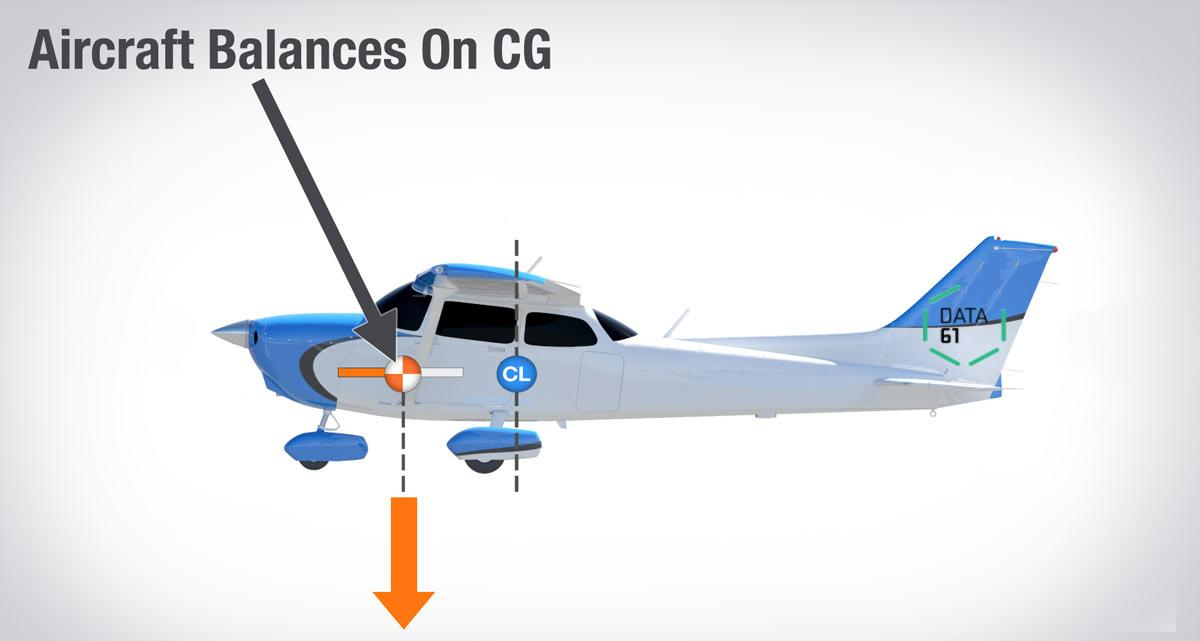
\includegraphics[height=0.5\textheight]{image/aircraft-cg.jpg}
\end{block}
\end{frame}

\begin{frame}
\frametitle{Fixed-wing Aircraft Weight and Balance}
\begin{block}{Same principles apply to A380}
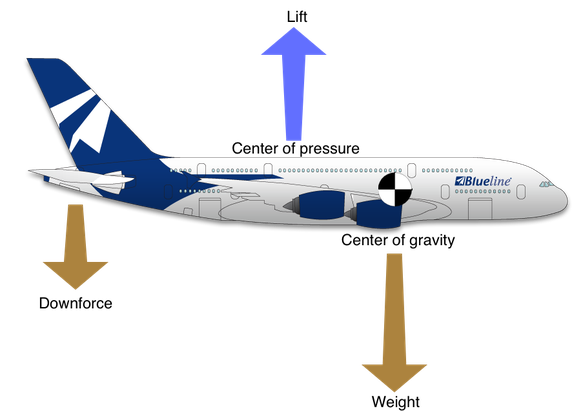
\includegraphics[height=0.5\textheight]{image/aircraft-cg-a380.png}
\end{block}
\end{frame}

\begin{frame}
\frametitle{Fixed-wing Aircraft Weight and Balance}
\begin{block}{Weight, Balance \emph{\tiny{loosely speaking}}}
\begin{itemize}
\item Weight is ensuring that the aircraft is able to achieve and maintain flight within parameters.
\item Balance is ensuring that the CG is positioned such that the aircraft is controllable.
\end{itemize}
\end{block}
\end{frame}

\begin{frame}
\frametitle{Fixed-wing Aircraft Weight and Balance}
\begin{block}{Calculating Weight and Balance}
\begin{itemize}
\item<1-> Obtain and normalise (to pounds) weights of
  \begin{itemize}
  \item \tiny{front seat PAX}
  \item \tiny{rear seat PAX}
  \item \tiny{baggage}
  \item \tiny{fuel/oil}
  \item \tiny{aircraft}
  \end{itemize}
\item<2-> Multiply each weight by the associated \emph{arm}.
\item<3-> Sum the products and plot the result on a flight envelope for that aircraft.
\end{itemize}
\end{block}
\end{frame}

\begin{frame}
\frametitle{Fixed-wing Aircraft Weight and Balance}
\begin{block}{CoG Moment Envelope}
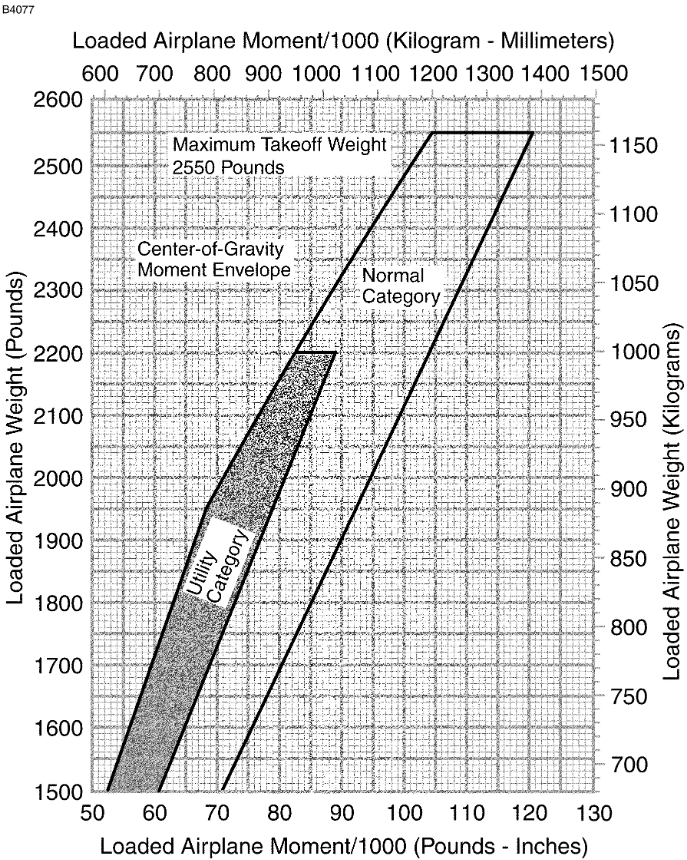
\includegraphics[height=0.8\textheight]{image/cg_moment_envelope.png}
\end{block}
\end{frame}

\begin{frame}
\frametitle{Fixed-wing Aircraft Weight and Balance}
\begin{block}{then this happens}
\begin{itemize}
\item<1-> Operator: ``We've changed your aircraft to VH-LSE.'' \emph{with a different empty weight}
\item<2-> Jessica: ``Hey is it cool if I sit in the front?''
\item<3-> There is now time pressure and distractions.
\item<3-> Start the calculation again, or use previous calculations and declare the difference insignificant.
\end{itemize}
\end{block}
\end{frame}

\begin{frame}
\frametitle{Fixed-wing Aircraft Weight and Balance}
\begin{block}{Computers can do this for us!}
\begin{itemize}
\item<1-> W\&B calculations are written in Haskell.
\item<2-> Jessica is a function argument and I can seat her anywhere, and immediately recalculate.
\item<3-> Different aircraft (and their weights) are function arguments.
\item<4-> Use diagrams package for plotting the flight envelope plot.
\end{itemize}
\end{block}
\end{frame}

\begin{frame}
\frametitle{Fixed-wing Aircraft Weight and Balance}
\begin{block}{Example result}
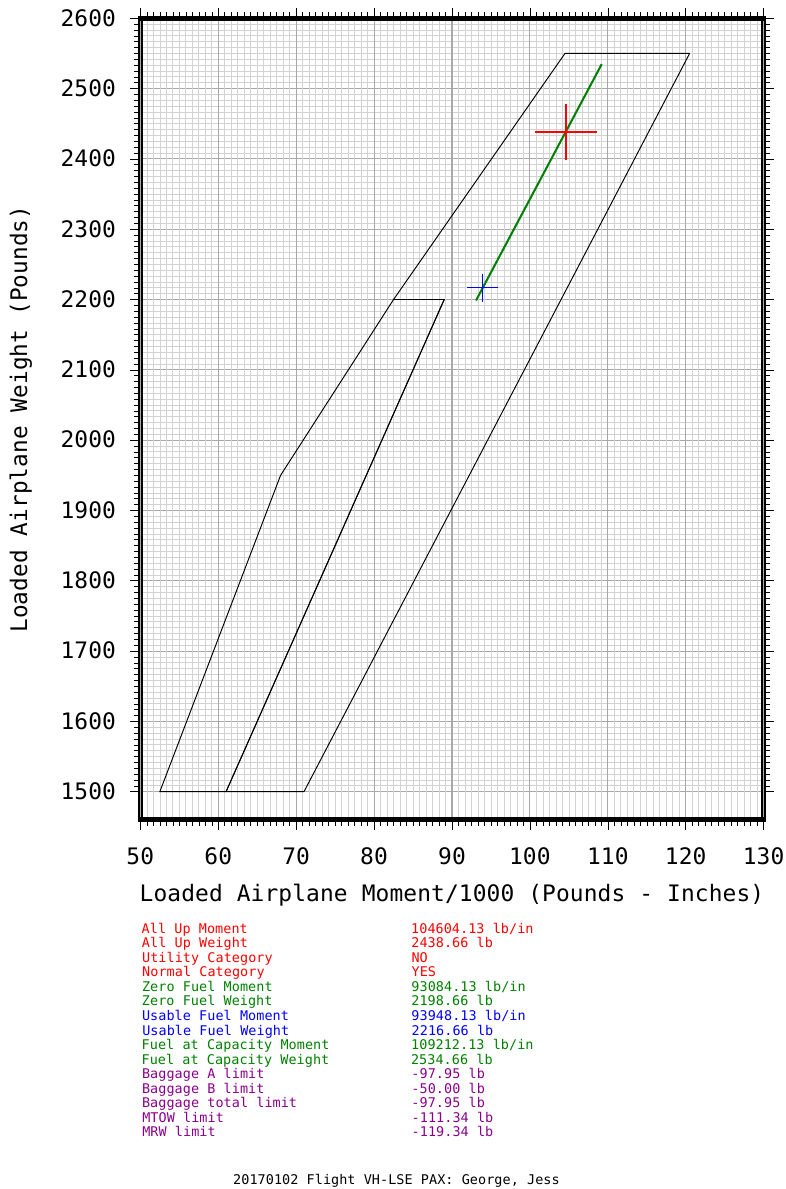
\includegraphics[height=0.8\textheight]{image/20170102-vhlse.png}
\end{block}
\end{frame}

\begin{frame}
\frametitle{Fixed-wing Aircraft Weight and Balance}
\begin{block}{}
W\&B calculations:
\begin{itemize}
\item<1-> are revision controlled
\item<2-> can be published as a library
\item<3-> can be queried retroactively
\end{itemize}
\end{block}
\end{frame}

\begin{frame}
\frametitle{Fixed-wing Aircraft Weight and Balance}
\begin{block}{Haskell source}
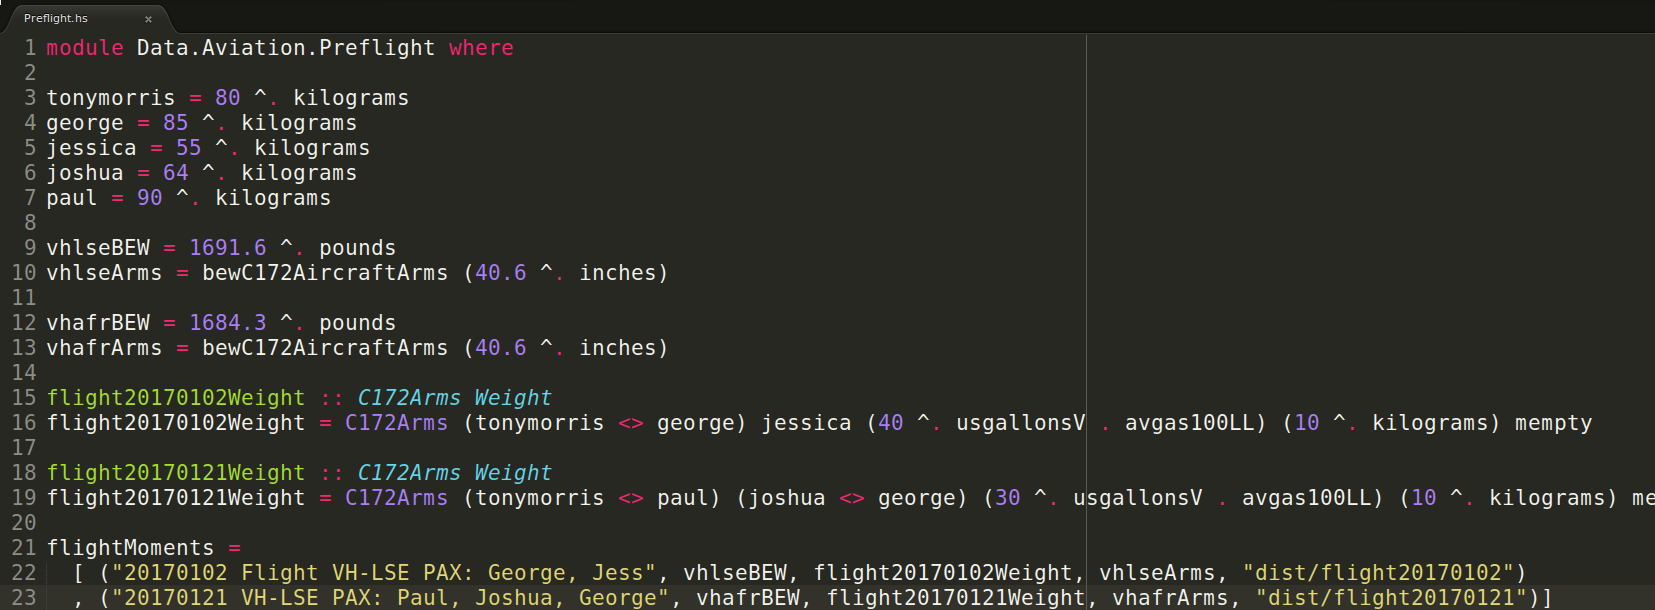
\includegraphics[height=0.44\textheight]{image/preflight-source.png}
\end{block}
\end{frame}
